% !Mode:: "TeX:UTF-8"% !TEX TS-program = xelatex
% !TEX encoding = UTF-8 Unicode
% !Mode:: "TeX:UTF-8"

%+++++++++++++++++++++++++++++++++++++++++++++++++++++++++++++++++++++++++++++
% This is a sample article script. All rights reserved.
% Author: qianhui@zju.edu.cn
%+++++++++++++++++++++++++++++++++++++++++++++++++++++++++++++++++++++++++++++
\documentclass[a4paper,twoside,AutoFakeBold]{article}
\usepackage{optreport}

%+++++++++++++++++++++++++++++++++++++++++++++++++++++++++++++++++++++++++++++
% Some packages for this sample.
%+++++++++++++++++++++++++++++++++++++++++++++++++++++++++++++++++++++++++++++
\usepackage{comment}	% Package for comment useless document
\usepackage{bm}			% Package for Bold-math symbol
\usepackage{mathrsfs}	% Package for RSFS fonts in maths
\usepackage{listings}	% Package for Listing code
\usepackage{enumerate}	% Package for enumerate
\usepackage{pdfrender}
\usepackage{subcaption}
\usepackage{multirow}
\usepackage{booktabs}
\usepackage{bbm}
\usepackage{bbding}
\usepackage{mathtools}
\usepackage{graphicx}
\usepackage{float}
\usepackage{epstopdf}
\usepackage{lipsum}
\usepackage{metalogo}
\usepackage{algorithm}
\usepackage{algorithmic}

%+++++++++++++++++++++++++++++++++++++++++++++++++++++++++++++++++++++++++++++
% Title, Authors, Reprot Time.
%+++++++++++++++++++++++++++++++++++++++++++++++++++++++++++++++++++++++++++++
\serialnum{2020-3-109315041}

\rptname{Optimal Transport Based Distributed \gaplongcap Optimization Research}

\rptauthora{周楠}{3220102535} %作者1和学号
\rptauthorb{王晓宇}{109315042} %作者2和学号
\rptauthorc{张三丰}{109315043} %作者3和学号
\reporttime{2024}{12}

% -------------------------------------------------
% for english version.
% -------------------------------------------------
\rptcontentsname{Contents}
\renewcommand{\abstractname}{{\xiaosan Abstract}}
\def\bibetal{et al.}
\def\biband{and}
\makeatletter
\renewcommand*{\ALG@name}{{\xiaosi Algorithm.~}}
\makeatother
\theoremstyle{definition}
\newtheorem{defn2}{{Definition}}
\newtheorem{corr2}{{Corrollary}}
\newtheorem{thrm2}{{Theorem}}
\newtheorem{lema2}{{Lemma}}
\newtheorem{exmp2}{{Example}}
\newtheorem{remark2}{{Remark}}
\renewcommand*{\proofname}{{\heiti Proof.~}}
\renewcommand{\figurename}{Fig.~}
\renewcommand{\tablename}{Tab.~}
\renewcommand{\refname}{Reference}
% -------------------------------------------------

%+++++++++++++++++++++++++++++++++++++++++++++++++++++++++++++++++++++++++++++
% Document.
%+++++++++++++++++++++++++++++++++++++++++++++++++++++++++++++++++++++++++++++
\begin{document}
\pagenumbering{gobble}

%-----------------------------------------------------------------------------
%  Title Page
%-----------------------------------------------------------------------------
\maketitle
\thispagestyle{empty} \clearpage

%-----------------------------------------------------------------------------
%  Table of Content
%-----------------------------------------------------------------------------
\rptcontent \thispagestyle{empty} \clearpage

%-----------------------------------------------------------------------------
%  Abstract
%-----------------------------------------------------------------------------
\begin{abstract}\kaiti \xiaosi
	We analyze Newton’s method with lazy Hessian
	updates for solving general possibly non-convex
	optimization problems. We propose to reuse a
	previously seen Hessian for several iterations
	while computing new gradients at each step of
	the method. This significantly reduces the overall
	arithmetic complexity of second-order optimiza-
	tion schemes. By using the cubic regularization
	technique, we establish fast global convergence
	of our method to a second-order stationary point,
	while the Hessian does not need to be updated
	each iteration. For convex problems, we justify
	global and local superlinear rates for lazy New-
	ton steps with quadratic regularization, which is
	easier to compute. The optimal frequency for
	updating the Hessian is once every d iterations,
	where d is the dimension of the problem. This
	provably improves the total arithmetic complexity
	of second-order algorithms by a factor $\sqrt{d}$.

	\vspace{2em}  % 增加 2em 的垂直间距


	我们分析了用lazy Hessian更新牛顿方法来解决一般的可能非凸优化问题。
	我们建议在方法的每一步计算新梯度的同时,在多次迭代中重复使用之前看到的 Hessian。
	这大大降低了二阶优化方案的整体算术复杂度。通过使用立方正则化技术,我们建立了我们的方法对二阶静止点的快速全局收敛性,
	同时不需要每次迭代更新赫赛安。对于凸问题,我们证明了使用二次正则化的懒牛顿步骤的全局和局部超线性率,这更容易计算。
	更新 Hessian 的最佳频率是每 d 次迭代一次,其中 d 是问题的维度。这可以证明,二阶算法的总算术复杂度提高了 $\sqrt{d}$ 倍。
\end{abstract}
\clearpage

%-----------------------------------------------------------------------------
%  Sections
%-----------------------------------------------------------------------------
\pagenumbering{arabic}\songti\xiaosi
%-----------------------
%
%-----------------------
\section{Introduction (引言)}

\subsection{章节组织}
\begin{enumerate}
    \item Introduction(引言): 介绍了二阶优化算法的背景和动机,特别是牛顿法在处理病态问题时的优势及其计算成本高的局限性。提出了惰性Hessian更新的核心思想,并概述了本文的主要贡献。
	\item Lazy Newton Steps(惰性牛顿步): 详细介绍了惰性牛顿步的定义和数学模型。通过在当前点计算梯度,而在过去的轨迹中使用Hessian矩阵,提出了带有立方正则化的惰性牛顿步。量化了二阶信息不精确性带来的误差,并形式化了单步方法的进展(定理2.1)。
	\item Global Convergence Rates(全局收敛性分析): 基于惰性牛顿步,提出了\textbf{带有惰性Hessian的立方牛顿法(Algorithm 1)},并证明了其快速全局收敛到二阶稳定点(定理3.1)。特别地,当Hessian每次迭代都更新时(\(m := 1\)),该方法恢复为经典的立方牛顿法。通过理论分析,证明了最优的Hessian更新频率是每\(d\)次迭代更新一次(\(m := d\)),从而将总复杂度提高了\(\sqrt{d}\)倍(推论3.6)。
	\item Minimizing Convex Functions(凸问题的优化): 针对凸问题,提出了\textbf{带有惰性Hessian的正则化牛顿法(Algorithm 2)},使用二次正则化替代立方正则化。这使得子问题更容易求解,仅涉及一次标准的矩阵求逆,同时保持了快速收敛速度。证明了该方法的全局复杂度与立方牛顿法相同,但每次迭代的计算成本更低。
	\item Local Superlinear Convergence(局部超线性收敛): 研究了新算法的局部收敛性,证明了这些算法在局部范围内具有超线性收敛速度(定理5.1和定理5.3)。特别地,对于经典牛顿法(无正则化),在惰性Hessian更新下也具有局部二次收敛性。
	\item Practical Implementation(实际实现): 讨论了算法的实际实现细节,包括矩阵分解和自适应搜索策略。提出了\textbf{自适应立方牛顿法(Algorithm 3)},通过动态调整正则化参数来进一步提高算法的性能。
	\item Experiments(实验): 通过数值实验验证了所提出方法的有效性。实验包括Soft Maximum问题、Logistic回归问题和对角神经网络训练问题。结果表明,惰性Hessian更新方法在保持收敛速度的同时显著减少了计算成本。
	\item Discussion(讨论): 总结了本文的主要贡献,并提出了未来可能的研究方向,包括研究具有特定Hessian结构的问题、探索惰性Hessian更新与拟牛顿法之间的联系,以及将分析推广到高阶优化方案。
\end{enumerate}

\subsection{问题背景}
在优化问题中,二阶优化算法(如牛顿法)在处理条件不佳问题时表现出色,
尤其是在局部范围内能够达到快速的二次收敛速度。然而,牛顿法的全局收敛性依赖于初始点的选择,
且每一步都需要计算梯度和Hessian矩阵,并进行矩阵分解,计算成本较高。
特别是在大规模问题中,Hessian矩阵的计算和存储成本非常高,这限制了牛顿法在实际应用中的广泛使用。

本文的核心动机是减少二阶优化算法的计算复杂度,特别是减少Hessian矩阵的计算频率。
作者提出了一种简单但有效的方法:惰性Hessian更新。
具体来说,算法在多次迭代中重用先前计算的Hessian矩阵,而每一步都使用新的梯度。
通过这种方式,可以显著减少Hessian矩阵的计算频率,从而降低总体的计算复杂度。

作者指出,Hessian矩阵的计算成本通常是梯度计算的d倍,其中d是问题的维度。
因此,通过减少Hessian矩阵的计算频率,可以显著加速算法的运行速度。
本文通过理论分析和实验验证,证明了惰性Hessian更新方法在保持收敛速度的同时,能够显著减少计算成本。

\subsection{相关工作}

惰性Hessian更新的思想并非全新,早在1967年,Shamanskii就提出了在非线性方程组求解中使用旧Hessian矩阵的局部收敛性分析。Shamanskii证明了在更新Hessian矩阵时,迭代具有局部二次收敛速度,而在不更新Hessian矩阵时,迭代具有线性收敛速度。

此后,这一思想被广泛应用于各种正则化方法中,如Levenberg-Marquardt正则化、阻尼牛顿步、近端牛顿法等。这些方法通常具有渐近全局收敛性,但没有显式的非渐近收敛速度保证。

本文的工作与这些方法的不同之处在于,作者使用了现代全局化技术(如立方正则化和梯度正则化),并证明了带有惰性Hessian更新的二阶优化算法在广泛的凸和非凸优化问题中具有快速的全局收敛速度。特别是,本文提出了非渐近的全局复杂度保证,证明了惰性Hessian更新方法在达到二阶稳定点时的全局复杂度为
$O(1/ε^{3/2})$
同时显著减少了Hessian矩阵的计算频率。

此外,本文还与最近提出的分布式牛顿型方法进行了对比。这些方法在联邦学习等场景中使用了Hessian矩阵的概率聚合和压缩技术。虽然这些方法也减少了Hessian矩阵的计算频率,但它们通常需要在每次迭代中评估Hessian矩阵,并根据某种准则决定是否使用新的Hessian矩阵。相比之下,本文的方法在每
$m$次迭代中只计算一次Hessian矩阵,从而进一步减少了计算成本。

\subsection{本文贡献}
\begin{enumerate}
    \item 提出了带有立方正则化的惰性牛顿步(第2节):
	该方法在当前点计算梯度,而在过去的轨迹中使用Hessian矩阵。量化了二阶信息不精确性带来的误差,并形式化了单步方法的进展(定理2.1)。
	展示了如何通过按比例增加正则化参数来平衡$m$次连续惰性牛顿步的误差。
	
	\item 基于此,开发了带有惰性Hessian的立方牛顿法(Algorithm 1),并证明了其快速全局收敛到二阶稳定点(第3节的定理3.1):
	这避免了方法陷入鞍点的问题。当$m:=1$(每次迭代都更新Hessian矩阵)时,方法恢复为经典的立方牛顿法(Nesterov \& Polyak, 2006)。
	
	在考虑Hessian计算的实际算术成本的情况下,方法的最优选择是每$m:=d$次迭代更新一次Hessian矩阵,从而将立方牛顿法的总复杂度提高了
	$\sqrt{d}$倍(见推论3.6)。
	
	\item 展示了如何在问题是凸问题时改进方法(第4节):
	开发了带有惰性Hessian的正则化牛顿法(Algorithm 2),它将模型中的立方正则化替换为二次正则化。这使得子问题更容易求解,仅涉及一次标准的矩阵求逆,同时保持了原始立方正则化方法的快速收敛速度。
	
	\item 研究了新算法的局部收敛性(第5节,见定理5.1和定理5.3):
	证明了这些算法都具有超线性收敛速度。作为一个特例,还证明了经典牛顿法(无正则化)在惰性Hessian更新下的局部二次收敛性。
	
	\item 提供了数值实验:
	通过数值实验验证了所提出方法的有效性。
\end{enumerate}




%-----------------------
%
%-----------------------
\section{Lazy Newton Steps (惰性牛顿步)}
惰性牛顿步的核心思想是重用先前计算的Hessian矩阵,而不是在每一步都重新计算。具体来说,算法在当前点计算梯度,而在过去的轨迹中使用Hessian矩阵。

惰性牛顿步的数学模型定义如下:
\[
Q_{\mathbf{x}, \mathbf{z}}(\mathbf{y}) = \langle \nabla f(\mathbf{x}), \mathbf{y} - \mathbf{x} \rangle + \frac{1}{2} \langle \nabla^{2}f(\mathbf{z})(\mathbf{y} - \mathbf{x}), \mathbf{y} - \mathbf{x} \rangle 
\]
\[
\mathbf{T}_{M}(\mathbf{x},\mathbf{z}) = \arg\min_{\mathbf{y}\in\mathbb{R}^{d}} 
\left\{ Q_{\mathbf{x}, \mathbf{z}}(\mathbf{y}) + \frac{M}{6} \|\mathbf{y} - \mathbf{x}\|^{3} \right\}
\]

\begin{itemize}
    \item \(\mathbf{x}\) 是当前点,\(\nabla f(\mathbf{x})\) 是在当前点计算的梯度。
    \item \(\mathbf{z}\) 是过去某次迭代的点,\(\nabla^{2}f(\mathbf{z})\) 是在该点计算的Hessian矩阵。
    \item \(M\) 是正则化参数,用于控制步长。
\end{itemize}

由于Hessian矩阵是过去某次迭代的计算结果,与当前点的Hessian矩阵可能存在差异,这种差异会引入误差。为了平衡这种误差,作者引入了\textbf{立方正则化},并通过增加正则化参数 \(M\) 来抵消误差的影响。

定义意味着点 \(\mathbf{T} = \mathbf{T}_{M}(\mathbf{x},\mathbf{z})\) 是立方正则化模型的全局最小值,尽管该模型通常是非凸的。然而,事实证明,可以使用最初为信任域方法开发的标准技术(Conn et al., 2000)高效地计算该点。

定义 \(r \stackrel{\text{def}}{=} \|\mathbf{T} - \mathbf{x}\|\)。\(\mathbf{T} = \mathbf{T}_{M}(\mathbf{x},\mathbf{z})\)的解满足以下平稳条件:

\[
\begin{cases}
\nabla f(\mathbf{x}) + \nabla^{2}f(\mathbf{z})(\mathbf{T} - \mathbf{x}) + \frac{M r}{2} \mathbf{B}(\mathbf{T} - \mathbf{x}) = \mathbf{0}, \\
\nabla^{2}f(\mathbf{z}) + \frac{M r}{2} \mathbf{B} \succeq 0.
\end{cases}
\]

因此,在非退化情况下,一步可以表示为以下形式:

\[
\mathbf{T} = \mathbf{x} - \left( \nabla^{2}f(\mathbf{z}) + \frac{M r}{2} \mathbf{B} \right)^{-1} \nabla f(\mathbf{x}),
\]

并且可以通过求解相应的单变量非线性方程(Nesterov \& Polyak, 2006, Section 5)找到值 \(r > 0\)。这可以通过预先计算的Hessian矩阵的特征值或三对角分解非常高效地完成。通常,其成本与经典牛顿步中的矩阵求逆相似。

定义以下量,对于 \(\mathbf{y} \in \mathbb{R}^{d}\):

\[
\xi(\mathbf{y}) \stackrel{\text{def}}{=} \left[ -\lambda_{\min} \left( \mathbf{B}^{-1/2} \nabla^{2}f(\mathbf{y}) \mathbf{B}^{-1/2} \right) \right]_{+},
\]

其中 \([t]_{+} \stackrel{\text{def}}{=} \max\{t, 0\}\) 表示正部,\(\lambda_{\min}(\cdot)\) 是对称矩阵的最小特征值。如果对于某个 \(\mathbf{y} \in \mathbb{R}^{d}\) 有 \(\nabla^{2}f(\mathbf{y}) \succeq 0\),则 \(\xi(\mathbf{y}) = 0\)。否则,\(\xi(\mathbf{y})\) 表示Hessian矩阵的最小特征值相对于固定矩阵 \(\mathbf{B} \succ 0\) 的大小(绝对值)。

\subsection*{定理 2.1}

设 \(M \geq L\)。那么,对于一次立方步$
\mathbf{T}_{M}(\mathbf{x},\mathbf{z}) = \arg\min_{\mathbf{y}\in\mathbb{R}^{d}} 
\left\{ Q_{\mathbf{x}, \mathbf{z}}(\mathbf{y}) + \frac{M}{6} \|\mathbf{y} - \mathbf{x}\|^{3} \right\}
$,有以下结论:
\[
f(\mathbf{x}) - f(\mathbf{T}) \geq \max \left\{ \frac{1}{648M^{2}} \xi(\mathbf{T})^{3}, \frac{1}{72\sqrt{2M}} \|\nabla f(\mathbf{T})\|_{*}^{3/2} \right\} + \frac{M}{48} r^{3} - \frac{11L^{3}}{M^{2}} \|\mathbf{z} - \mathbf{x}\|^{3}.
\]

定理2.1展示了可以从一次带有立方正则化的惰性牛顿步中期望的进展。使用惰性Hessian的代价是最后一项,如果 \(\mathbf{z} := \mathbf{x}\)(为当前迭代更新Hessian矩阵),则该项消失。


\section{Global Convergence Rates(全局收敛性分析)}


\newpage
\section{Minimizing Convex Functions(凸问题的优化)}
在凸优化问题中,目标函数的Hessian矩阵是半正定的(即 \(\nabla^{2}f(\mathbf{x}) \succeq 0\))。这使得可以使用更简单的正则化技术来简化子问题的求解。本文针对凸问题,提出了\textbf{带有惰性Hessian的正则化牛顿法(Algorithm 2)},使用二次正则化替代立方正则化,从而使得子问题更容易求解。

\begin{algorithm}
\caption{Regularized Newton with Lazy Hessians}
\label{alg:reg_newton_lazy_hessians}
\begin{algorithmic}[2]
\REQUIRE $\mathbf{x}_{0} \in \mathbb{R}^{d}$, $m \geq 1$, $L > 0$
\ENSURE Sequence $\{\mathbf{x}_{k}\}_{k \geq 0}$ converging to a second-order stationary point

\STATE Choose $M := 3mL$ \COMMENT{Set regularization parameter}
\FOR{$k = 0, 1, \ldots$}
	\STATE Set last snapshot point $\mathbf{z}_{k} = \mathbf{x}_{\pi(k)}$ \COMMENT{Reuse Hessian from $\pi(k)$-th iteration}
	\STATE Compute $\lambda_{k} = \sqrt{M \|\nabla f(\mathbf{x}_{k})\|_{*}}$ \COMMENT{Compute regularization parameter}
	\STATE Compute lazy Newton step:
	\[
	\mathbf{x}_{k+1} = \mathbf{x}_{k} - \left( \nabla^{2}f(\mathbf{z}_{k}) + \lambda_{k} \mathbf{B} \right)^{-1} \nabla f(\mathbf{x}_{k})
	\]
\ENDFOR
\end{algorithmic}
\end{algorithm}
算法2的全局复杂度界与算法1的复杂度界相同(最多相差一个对数项)。然而,算法2的每次迭代更容易实现,因为它仅涉及求解一个线性系统。
\begin{itemize}
    \item \textbf{迭代次数}:达到精度 \(\|\nabla f(\mathbf{x}_{k+1})\|_{*} \leq \varepsilon\) 所需的迭代次数为:
    \[
    k \leq \mathcal{O}\left( \frac{\sqrt{m} L (f(\mathbf{x}_{0}) - f^{*})}{\varepsilon^{3/2}} + \ln \frac{\|\nabla f(\mathbf{x}_{0})\|_{*}}{\varepsilon} \right).
    \]
    \item \textbf{Hessian更新次数}:在达到精度 \(\varepsilon\) 的过程中,Hessian矩阵的更新次数为:
    \[
    t \leq \mathcal{O}\left( \frac{\sqrt{L} (f(\mathbf{x}_{0}) - f^{*})}{\varepsilon^{3/2} \sqrt{m}} + \frac{1}{m} \ln \frac{\|\nabla f(\mathbf{x}_{0})\|_{*}}{\varepsilon} \right).
    \]
\end{itemize}
\section{Local Superlinear Convergence(局部超线性收敛)}


\section{Practical Implementation(实际实现)}

\newpage
\section{Experiments(实验)}

通过数值实验展示了所提出的带有惰性Hessian更新的二阶方法的性能。考虑以下凸最小化问题,目标函数为\textbf{Soft Maximum}(log-sum-exp):
\[
\min_{\mathbf{x} \in \mathbb{R}^{d}} f(\mathbf{x}) := \mu \ln \left( \sum_{i=1}^{n} \exp \left( \frac{\langle \mathbf{a}_{i}, \mathbf{x} \rangle - b_{i}}{\mu} \right) \right) \approx \max_{1 \leq i \leq n} \left[ \langle \mathbf{a}_{i}, \mathbf{x} \rangle - b_{i} \right].
\]

为了生成数据,随机采样向量 \(\bar{\mathbf{a}}_{1}, \ldots, \bar{\mathbf{a}}_{n} \in \mathbb{R}^{d}\) 和 \(\mathbf{b} \in \mathbb{R}^{n}\),元素来自 \([-1, 1]\) 的均匀分布。然后,我们使用这些向量构建辅助目标函数 \(\bar{f}\),并设置 \(\mathbf{a}_{i} := \bar{\mathbf{a}}_{i} - \nabla \bar{f}(\mathbf{0})\)。这确保了最优解位于原点,因为 \(\nabla f(\mathbf{0}) = \mathbf{0}\)。初始点为 \(\mathbf{x}_{0} = (1, \ldots, 1)\)。

对于原始范数(2),使用矩阵:
\[
\mathbf{B} := \sum_{i=1}^{n} \mathbf{a}_{i} \mathbf{a}_{i}^{\top} + \delta \mathbf{I} \succ 0,
\]

其中 \(\delta > 0\) 是一个小的扰动参数,用于确保正定性。然后,Hessian矩阵的Lipschitz常数由以下公式界定:\(L = 2 / \mu^{2}\),其中 \(\mu > 0\) 是平滑参数。

由于问题是凸的,我们可以应用带有梯度正则化的牛顿法(Algorithm 2)。在图1中,比较了不同参数 \(m\) 值(即Hessian更新的频率)的性能。正则化参数固定为 \(M := 1\)。还展示了梯度法(Gradient Method, GM)作为标准基线的性能。

\begin{figure}[H]
    \centering
    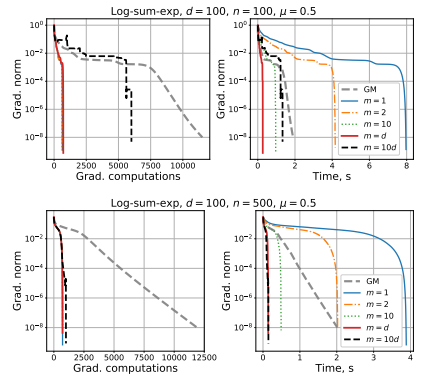
\includegraphics[width=0.8\textwidth]{figs/1.png}
    \caption{Hessian更新频率对算法性能的影响}
    \label{fig:fig1}
\end{figure}

实验结果表明:

1. 通过增加Hessian更新的频率(即增加$m$的值),可以显著提高算法的总体性能。最优的更新频率是 
$m=d$,这与理论分析一致。

2. 与每次迭代都更新Hessian矩阵的经典牛顿法相比,惰性Hessian更新方法在保持收敛速度的同时,显著减少了计算成本。

3. 二阶方法(如立方牛顿法和正则化牛顿法)在收敛速度和计算效率上均优于经典的梯度法。



\newpage
\section{Discussion(讨论)}

\subsection{结论}

在本文中,开发了新的带有\textbf{惰性Hessian更新}的二阶优化算法,用于解决一般的非凸优化问题。展示了在多次迭代中重用先前计算的Hessian矩阵可以显著提高算法的效率,而不需要每次迭代都更新Hessian矩阵。

通过使用\textbf{立方正则化}和\textbf{梯度正则化}技术,证明了带有惰性Hessian更新的二阶方法在广泛的凸和非凸优化问题中具有快速的全局和局部收敛速度。证明了最优的Hessian更新策略是每 \(d\) 次迭代更新一次Hessian矩阵,其中 \(d\) 是问题的维度。这显著减少了二阶算法的总算术复杂度,提高了 \(\sqrt{d}\) 倍。
\subsection{未来工作方向}
作者提出了以下几个未来可能的研究方向:
\begin{enumerate}
    \item \textbf{特定Hessian结构的研究}:研究具有特定Hessian结构(如稀疏性或某些谱聚类)的问题,可能需要不同的Hessian更新策略。
    \item \textbf{与拟牛顿法的联系}:探索惰性Hessian更新与经典拟牛顿法之间的联系。拟牛顿法通过逐步更新Hessian矩阵的近似来优化问题。
    最近发现的拟牛顿法的非渐近复杂度界限(Rodomanov \& Nesterov, 2021; Rodomanov, 2022)可能对实现这一目标特别有用。
    \item \textbf{高阶优化方案的推广}:将分析推广到高阶优化方案(Nesterov, 2021)。高阶方法使用更高阶的导数信息来加速收敛。
	主要挑战是如何高效地重用高阶张量,这可能需要使用一些高级的张量分解技术。
    \item \textbf{凸优化的进一步研究}:在凸优化中,除了梯度范数外,另一个常见的精度度量是函数残差。
	可能可以证明使用函数残差作为度量时,惰性Hessian更新方法具有更好的收敛速度。还可以研究加速和超通用的二阶方法。
\end{enumerate}



%+++++++++++++++++++++++++++++++++++++++++++++++++++++++++++++++++++++++++++++
% Bibliography
%+++++++++++++++++++++++++++++++++++++++++++++++++++++++++++++++++++++++++++++
\bibliographystyle{gbt7714-plain}
\bibliography{main}

%+++++++++++++++++++++++++++++++++++++++++++++++++++++++++++++++++++++++++++++
\end{document}
%+++++++++++++++++++++++++++++++++++++++++++++++++++++++++++++++++++++++++++++


